\documentclass{IEEEtran}
\usepackage{bm}
\usepackage{amsmath}
\usepackage{amssymb}
\usepackage{algorithm}
\usepackage{algorithmicx}
\usepackage{algpseudocode}
\usepackage{graphicx}
\DeclareMathOperator*{\argmax}{arg\,max}
\DeclareMathOperator*{\argmin}{arg\,min}
\DeclareMathOperator*{\sigmoid}{sigmoid}

\renewcommand{\IEEEQED}{\IEEEQEDclosed}
\title{Optimal Fishing Strategy Based on Scientific Concept of Development}
\author{
    Weitong~ZHANG, Yiwen~LU, Zifeng~KANG*
    \thanks{Weitong~ZHANG 2015011493 Email: \texttt{WeightZero@outlook.com}}
    \thanks{Yiwen~McF.~LU 2015011443 Email: \texttt{ylu.thu15@gmail.com}}
    \thanks{Zifeng~KANG 2015011??? Email: \texttt{scikit-learn@python.org}}
}
\begin{document}
\maketitle

\begin{abstract}
    The SOD incorporates scientific socialism, sustainable development, social welfare, a humanistic society, increased democracy, and, ultimately, the creation of a Socialist Harmonious Society. According to official statements by the CPC, the concept integrates "Marxism with the reality of contemporary China and with the underlying features of our times, and it fully embodies the Marxist worldview on and methodology for development."
\end{abstract}

\section{Introduction}

With the rapid growth of modern society and technology, the depletion of resources has brought about jarring problems to environmentalists, economists and policy makers, and even serious threats to the survival of human beings. Even today, in most countries, how to rationally develop and use resources still remains a vital issue that requires collaboration of country leaders with ordinary people.

Fortunately, faced with this tough situation, leaders of Communist Party of China have proposed Scientific Concept of Development (SCD). The basic requirements of SCD are comprehensive, coordinated, and sustainable. In the light of SCD, development of our country aims to ensure profitability while maintain sustainability.

Thoughts of SCD are so inclusive and universal that we decided to apply them to fishery problems. As a renewable kind of resource, fish die and spawn hatch at a speed that we are able to calculate and predict. In order to provide practical advice to fishermen, previous studies have found that fixed-effort-capture strategy can both ensure profitability while maintain sustainability. We developed two state-of-the-art models in this paper.

\section{Basic Assumptions}
\subsection{Features of Fish}
\begin{itemize}
\item {The maturing time period of involved fish is exactly 4 years, which means when the next year arrives, alive spawns of the first year hatch into 1-aged fish and alive $i$-aged fish grow into $(i+1)$-aged fish($i=1,2,3$), while alive 4-aged fish remain 4-aged.}
\item {Fish that share the same age are homogeneous, including weight, size, growth and spawning behavior and possibility to be captured.}
\item {The amount of each fish group is continuously differentiable as a function of time.}
\item {All fish die at all times at a constant speed, with a total annual natural fatal rate of 0.8 .}
\item {All fish spawn instantaneously, and all spawns are homogeneous. }
\end{itemize}

\subsection{Features of Human Captures}
\begin{itemize}
\item {Human capture fish at all times at a speed proportional to fish amount at that time. The proportion coefficient is called \textit{fishing intensity}.}
\item {At the end of each year, if remaining fish of each group are not less than 80\% of saturation level, then in that year `fish productivity is not badly damaged'.}
\end{itemize}
\section{Model on Sustainable Harvesting} \label{model1}
Owing to the annual death ratio is 0.8, we assume that the number of fish $x$ obeys the distribution eq. \ref{eq1}

\begin{equation}
    \label{eq1}
    x = x_0 \exp(-\lambda t)
\end{equation}

while the unit of $t$ is year, we get $\lambda = \ln 5, \frac{\mathrm dx}{\mathrm dt} = -\lambda x$

Setting the fishing intensity of 4-aged fish to be $k$, we can get the one of 3-aged fish is $0.42k$, while the number of the four group of fish could be described as a 4-d vector $\bm x$ .

\subsection{Model on the first eight months}

We can use the differential equation eq. \ref{eq2} to describe the trend of the number of fish in each group

\begin{align}
    \label{eq2}
    -\frac{\mathrm d \bm x}{\mathrm d t} &= k \mathbf C \bm x + \lambda \bm x \\
    \mathbf C &= \begin{pmatrix}0&0&0&0\\0&0&0&0\\0&0&0.42&0\\0&0&0&1\end{pmatrix}
\end{align}
\subsection{Model on the last four months}
Set the number of eggs is $y$, and for each fish, we set the rate of spawning is $\mu$, i.e. $\frac {\mathrm d y_i}{\mathrm d t} = \mu$, where $y_i$ is the eggs spawned by a certain fish $i$. Then we get the following differential equation eq. \ref{eq3}

\begin{align}
    \label{eq3}
    \frac {\mathrm d y}{\mathrm d t} &= \mu \mathbf D \bm x\\
    -\frac{\mathrm d \bm x}{\mathrm d t} &=\lambda \bm x\\
    \mathbf D &= \begin{pmatrix} 0 & 0 & 1.109\times10^5/2&1.109\times10^5\end{pmatrix}
\end{align}

From the average spawning rate, we can get that $\mu = 3$.

\subsection{Model on the changes of the next year}

After a year, some eggs spawned in the first year would be the 1-aged fish, according to the survival ratio. Therefore, we can get the following transform function eq. \ref{eq4}

\begin{align}
    \label{eq4}
    y &= 0\\
    \bm x &= \mathbf T \bm x +\begin{pmatrix} f(y)&0&0&0\end{pmatrix}^{\mathrm T}\\
    f(y) &= \frac{1.22\times 10 ^{11}y}{1.22\times 10 ^{11} + y}\\
    \mathbf T &= \begin{pmatrix} 0 & 0 & 0 & 0 \\ 1& 0 & 0 & 0 \\ 0 & 1 & 0 & 0 \\0 & 0 & 1 & 1 \end{pmatrix}
\end{align}

\subsection{Solve the function}

Now We can conclude all of the function above to solve the equation \ref{eq5} of $\bm x$: $\bm x' = \bm x$ based on $k$, where $\bm x'$ is the number of fish next year:  

\begin{align}
    \bm x' &= \bm x_0\\
    \label{eq5}
    \bm x' &= \mathbf T \exp(-\frac{\mathbf A_2 + 2 \mathbf A_1}{3})\bm x_0 +\begin{pmatrix} f(\mathbf B \exp(-\frac{2\mathbf A_1}{3})\bm x_0)\\0\\0\\0\end{pmatrix}
\end{align}
\begin{align}
    \mathbf A_1 &= k\mathbf C + \lambda \mathbf I\\
    \mathbf A_2 &= \lambda \mathbf I\\
    \mathbf B &= (\mu \mathbf D A_2^{-1}(\mathbf I - \exp(-\mathbf A_2/3)))
\end{align}

Therefore, we can get the relationship between $\bm x$ and $k$ numerically.
\subsection{Relation bewteen Harvest and Fishing Intensity}
The total of harvest $z$ could be described as the following function eq. \ref{eq6}

\begin{align}
    \label{eq6}
    \frac {\mathrm dz}{\mathrm dt} &= k\mathbf C \vec x\\
    z &= k\mathbf C\int_0^{2/3}\exp(-\mathbf A_1t)\mathrm dt\bm x_0 \\ 
    &= k\mathbf C  A_1^{-1} (1-\exp(-2\mathbf A_1/3))\bm x_0
\end{align}

where $\bm x_0$ would be the initial number of fish.


%%%%%%%%%%%%%%%%%%%%%%%%%%%%%%%%%%%%%%%%%
%
%         RESULT FOR PART 1
%
%%%%%%%%%%%%%%%%%%%%%%%%%%%%%%%%%%%%%%%%%
\section{Model on five successive fishing}

According to the analysis above, we can also calculate the number of fish $\bm x'$ in the next year by eq.\ref{eq5}, and we can also get the sum of the harvest $z$, let's set the relationship between them as eq. \ref{eq7}

\begin{equation}
    \label{eq7}
    \bm x' = F(\bm x, k), \bm z = G(\bm x,k)
\end{equation}

Therefore, the total harvest and the number of fish remaining after 5 years could be calculate by the following algorithm \ref{A1}

\begin{algorithm}[h]
    \caption{Calculate the harvest and the number of fish}\label{A1}
    \begin{algorithmic}
        \Require Initial state $\bm X_0$, fishing strategy $\bm K = [k_1,\cdots,k_5]$ 
        \Ensure Sum of harvest $Z$ and the number of fish after 5 years $\bm X$
        \State Let $\bm X = \bm X_0, Z = 0$
        \For{$i$ in $[1,\cdots,5]$}
        \State $Z \Leftarrow Z + G(\bm X,\bm K_i)$
        \State $\bm X \Leftarrow F(\bm X, \bm K_i)$
        \EndFor
    \State \Return $Z$ and $\bm X$
    \end{algorithmic}
\end{algorithm}

According to the contract, the productive ability could not be bitterly destroyed after 5 years. However, this rule is a relatively blurry one, which needs a quantitative description. In the following discussing, we will try several method to decide the factor $\Gamma \le 1$, which is used to describe the loss of the productive ability. And our objective function would be $H(\bm K) = Z\Gamma$, while $Z$ is calculated by algorithm \ref{A1}. We are about to maximize $H(\bm K)$

\subsubsection{Baseline of productive ability}

First of all, we need to provide a baseline of productive ability. It is reasonable to guess that the maximum of the number of fish is the steady state with $k = 0$, according to the survival rate of the eggs, we can guess that the 1-aged fish is limited to the following value:

\begin{equation}
    x_1 = \lim_{y\to\infty} f(y) = 1.22 \times 10^{11}
\end{equation}

Using this value as the 1-aged fish, we can conclude that the saturation of the number of fish is obeying the following function:

\begin{equation}
    \begin{cases}
        x_2 = 0.2 x_1\\
        x_3 = 0.2^2 x_1\\
        x_4 = 1.25 \times 0.2^3 x_1
    \end{cases}
\end{equation}

Therefore, the saturation of the number of fish should be described as eq. \ref{eq8}

\begin{equation}
    \label{eq8}
    \bm X_s = 1.22 \times 10^{11}\begin{pmatrix}1 & 0.2 & 0.04 & 0.01\end{pmatrix}^\mathrm T
\end{equation}

\subsubsection{Penalty I. Comparison with the saturation number of fish}

It is obvious that it is a good idea to keep the number of the fish similar to the saturation one $\bm X_s$, therefore, we can design our object function as eq. \ref{eq9}

\begin{align}
    \label{eq9}
    \Gamma &= \sigmoid(\frac{(\Theta^\mathrm T)(\bm X / \bm X_s - 0.8)}{\sigma})
\end{align}

Where $\sigma$ and $\Theta$ are designed manually, $\Theta$ is a $4 \times 1$ vector, and the division $\bm X / \bm X_s$ is the element-size devision. $\bm X$ and $Z$ could be calculate by symbolic computation in algorithm \ref{A1}

The sigmoid function should be described as eq. \ref{eq10}

\begin{equation}
    \label{eq10}
    \sigmoid(x) \triangleq \frac1{1 + \exp(-x)}
\end{equation}

We are about to maximize the $H(\bm K)$, and it is obvious that if the final number of fish $\bm X$ is much closer to $\bm X_s$, the $H(\bm K)$ would be also increasing.

\subsubsection{Optimizer: the Gradient Descent method}

By using computer algebra method, we can easily get the derivative of the object function, i.e. $\frac{\partial H}{\partial \bm K}$, and therefore we could use GD method to get the better fishing strategy.

%%%%%%%%%%%%%%%%%%%%%%%%%%%%%%%%%%%%%%%%%%%%%%%%%%%%%%%%%%%%%%%%%%
%
%              RESULT FOR G.D. METHOD
%
%%%%%%%%%%%%%%%%%%%%%%%%%%%%%%%%%%%%%%%%%%%%%%%%%%%%%%%%%%%%%%%%%%%

\subsubsection{Other Optimizer and Other Penalty Functions}

The penalty mentioned above is focus on the changing of the numbers, however, it is also possible that different combinations of numbers can gain the same productive ability. Therefore, the penalty here is more curious about the total harvest in the later years.

\begin{itemize}
    \item {Short Term Assess Method

    By running the body of the loop in algorithm \ref{A1}, we can calculate the harvest of the next year $Z'(k) = G(\bm X,k)$, let the penalty factor $\Gamma$ be eq. \ref{eq11}
    
    \begin{equation}
        \label{eq11}
        \Gamma \triangleq \min_{k \in[1,2,\cdots,20]} \frac{G(\bm X,k)}{G(\bm X_s,k)}
    \end{equation}
    }

    \item {Long Term Assess Method
        
    According to the further analysis, however, the short term assess method do not sound like a good idea, which is because the productive ability described by this method cannot take the 1-aged fish and 2-aged fish into consideration for it is only consider the next year, when the 1-aged one and 2-aged one are not abot to spawn. Hence, we need to expand the short-term method into a relatively long-term method. For the reason that the periodic time of the fish is about 4 years, we use the 4-year-term should be better. The $\Gamma$ function should be desctibed as eq. \ref{eq12}, in which we calculate the total harvest by algorithm \ref{A1} (or a relatively similar algorithm) and set the result with the initial state $\bm X$ and intensity (which is constant during the 4 years) $k$ as $R(\bm X,k)$
    
    \begin{equation}
        \label{eq12}
        \Gamma \triangleq \min_{k \in[1,2,\cdots,20]} \frac{R(\bm X,k)}{R(\bm X_s,k)}
    \end{equation}
    In which the total harvest could be calculated also by algorithm \ref{A1}.

    Further experiment shows that while it is inaccurate, it is also not a good idea to choose a much longer period, owing to the fact that the harvest in the last few years and the number of the fish then will arrive at a relatively stable state, which would cover the initial loss. In a few words, a 4-year-term is a good idea.
        }
\end{itemize}

For the two $\Gamma$ function based on harvest mentioned above, the optimization based on gradient might not sound like a good idea, therefore, we use MATLAB\textsuperscript\textregistered \ toolbox to solve this problems. By using functions like fmincon (which is based on the calculated gradient), and GA (which completely treat the object function as a blackbox), the optimization process performs well and generate the result just like we want.

\section{Result}

\subsection{Solution to the first problem}

Applying the model described in Part \ref{model1}, under the constraint of sustainable harvesting, the annual harvest $z$ can be represented as a function w.r.t. the fishing intensity of 4-aged fish $k$. The analytical expression is derived with SymPy \footnote{Joyner, D., Certik, O., Meurer, A., \& Granger, B. E. (2012). Open source computer algebra systems: \textit{SymPy. ACM Communications in Computer Algebra, 45}(3/4), 225-234.}. The function is numerically plotted in Figure \ref{plot1}. Note that $z$ is meaningful if and only if $z>0$, and thus the feasible region of $k$ is automatically determined.

\begin{figure}[h]
	\centering
	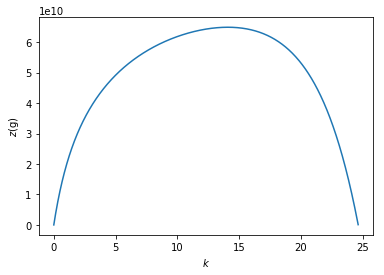
\includegraphics[width=\columnwidth]{plot1}
	\caption{The relationship between annual harvest $z$ and fishing intensity $k$\label{plot1}}
\end{figure}

The relationship between $z$ and $k$ is not monotonous, which agrees with our intuition: when $k$ is too small, the fishing intensity is too small to exploit the resources; when $k$ is too large, the number of fishes in the steady state is decreased, affecting the harvest. By performing a linear search on $k$, the optimal fishing strategy can be determined:

$$\begin{cases}\argmax\limits_k z(k) \approx 14.09\\\max\limits_k z(k) \approx 6.49\times 10^{10} \end{cases}$$

\subsection{Solution to the second problem using Gradient Descent}
\subsection{Solution to the second problem using other Optimizer}
17.3831   12.0797    9.4566   30.0000    0.0001
17.6717   14.1999   12.0285   11.4857   11.1067
\section{Conclusion}
\end{document}